\documentclass[a0paper,portrait]{baposter}

%----------------------------------------------------------------------------------------
%	SIMPLE BOXED ENVIRONMENT
%----------------------------------------------------------------------------------------

\usepackage{wrapfig}
\usepackage{lmodern}

\usepackage[utf8]{inputenc} %unicode support
\usepackage[T1]{fontenc}
\usepackage{amsmath}

\selectcolormodel{cmyk}

\graphicspath{{figures/}} % Directory in which figures are stored


\newcommand{\compresslist}{%
\setlength{\itemsep}{0pt}%
\setlength{\parskip}{1pt}%
\setlength{\parsep}{0pt}%
}

\newenvironment{boenumerate}
  {\begin{enumerate}\renewcommand\labelenumi{\textbf\theenumi.}}
  {\end{enumerate}}

% kaobox (while tcolorbox may be more rich, I find it too complicated so I prefer mdframed)
\RequirePackage{tikz}
\RequirePackage[framemethod=TikZ]{mdframed}

%\mdfsetup{skipabove=\topskip,skipbelow=0pt}
\mdfdefinestyle{kaoboxstyle}{
	skipabove=1.5\topskip,
	skipbelow=.5\topskip,
	rightmargin=0pt,
	leftmargin=0pt,
	%innertopmargin=3pt,
	%innerbottommargin=3pt,
	innerrightmargin=7pt,
	innerleftmargin=7pt,
	topline=false,
	bottomline=false,
	rightline=false,
	leftline=false,
	%linewidth=1pt,
	%roundcorner=0pt,
	%font={},
	%frametitlefont={},
	frametitlerule=true,
	linecolor=black,
	%backgroundcolor=LightBlue,
	fontcolor=black,
	%frametitlebackgroundcolor=LightBlue,
}

\newmdenv[
	style=kaoboxstyle,
	backgroundcolor=lightgreen!25,
	frametitlebackgroundcolor=lightgreen!25,
]{kaobox}


\begin{document}


\definecolor{darkgreen}{cmyk}{0.8,0,0.8,0.45}
\definecolor{lightgreen}{cmyk}{0.8,0,0.8,0.25}

\begin{poster}
{
grid=false,
headerborder=open, % Adds a border around the header of content boxes
colspacing=1em, % Column spacing
bgColorOne=white, % Background color for the gradient on the left side of the poster
bgColorTwo=white, % Background color for the gradient on the right side of the poster
borderColor=darkgreen, % Border color
headerColorOne=lightgreen, % Background color for the header in the content boxes (left side)
headerColorTwo=lightgreen, % Background color for the header in the content boxes (right side)
headerFontColor=white, % Text color for the header text in the content boxes
boxColorOne=white, % Background color of the content boxes
textborder=rounded, %rectangle, % Format of the border around content boxes, can be: none, bars, coils, triangles, rectangle, rounded, roundedsmall, roundedright or faded
eyecatcher=false, % Set to false for ignoring the left logo in the title and move the title left
headerheight=0.11\textheight, % Height of the header
headershape=rounded, % Specify the rounded corner in the content box headers, can be: rectangle, small-rounded, roundedright, roundedleft or rounded
headershade=plain,
headerfont=\Large\textsf, % Large, bold and sans serif font in the headers of content boxes
%textfont={\setlength{\parindent}{1.5em}}, % Uncomment for paragraph indentation
linewidth=2pt % Width of the border lines around content boxes
}
{}
%
%----------------------------------------------------------------------------------------
%	TITLE AND AUTHOR NAME
%----------------------------------------------------------------------------------------
%
{
\textsf %Sans Serif
{A Pumped Hydroelectric Storage Option in France?
}
} % Poster title
% {\vspace{1em} Marta Stepniewska, Pawel Siedlecki\\ % Author names
% {\small \vspace{0.7em} Department of Bioinformatics, Institute of Biochemistry and Biophysics, PAS, Warsaw, Pawinskiego 5a}} % Author email addresses
{\sf\vspace{0.5em}\\
A long term outlook on the physical challenges of developing pumped hydroelectric storage.
}
{
\includegraphics[width=35mm,scale=0.35]{favpng_question-mark-logo-information}} % University/lab logo


\headerbox{1. Case Study}{name=introduction,column=0,row=0, span=3}{
When the arguments against batteries come, such as the price or materials availability, it is customary to move the problem of energy storage to pumped hydroelectric storage. After all, it represents 95\% of all energy storage capacity in the world today, and has been proven to work for decades. In this case study, we will assess what this would imply in terms of engineering to meet France storage requirements in a 100\% renewable mix scenario with this technology.
}


\headerbox{2. Energy Storage}{name=model,column=0,below=introduction,span=1}{

In this very simple development, we will use the current energy needs, extrapolated to be constant over the next century. We will also assume that gaining efficiency on the heat conversion process of current gas-powered machines will show significant savings. In terms of share of production, this scenario looks at the transition from today's energy mix to 50\% solar, and 50\% wind (both onshore and offshore).

\begin{center}
    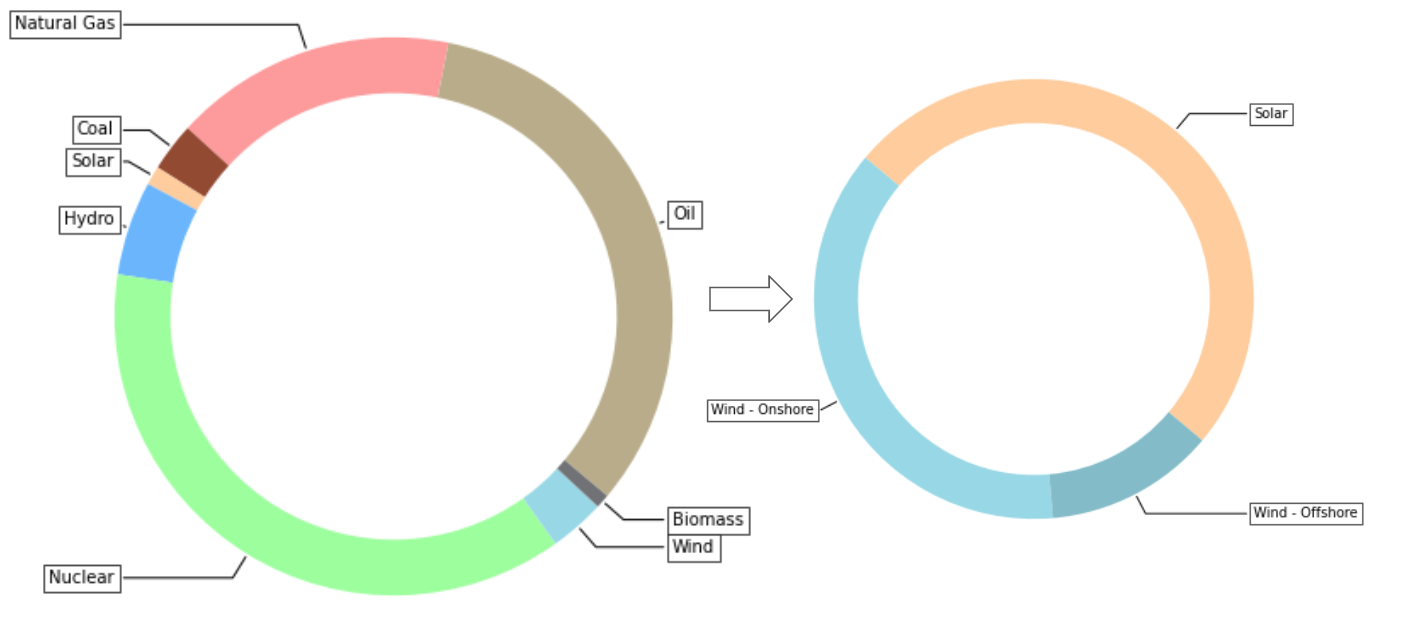
\includegraphics[width=\linewidth]{transition_s2a_smaller}
%$\big\Downarrow$
%    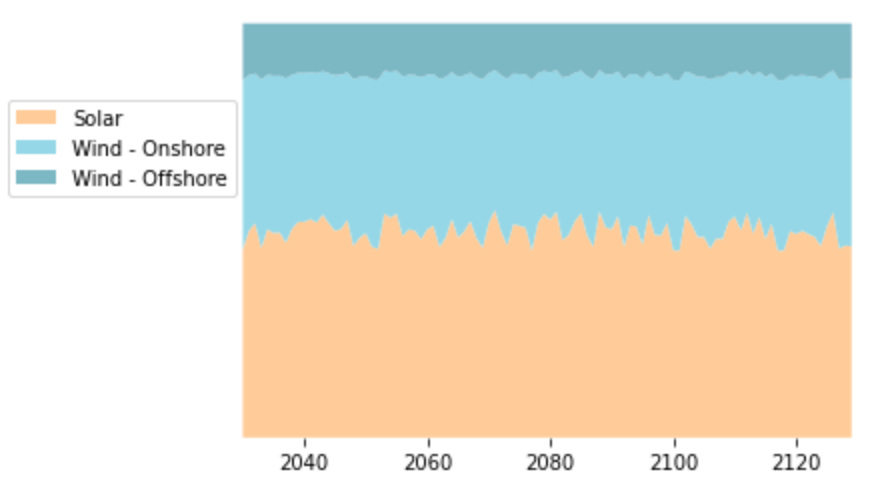
\includegraphics[width=\linewidth]{future_mix_s2a}
\end{center}
%\vspace{-2pt}

We assume an energy consumption of 2,800 TWh (approximate current value in France), and decrease it down to 2,000 TWh to account for the better electrical efficiency of non-heat conversion systems.

As we have discussed, we can hope, in a very optimistic scenario, to only need to backup 10\% of our consumption needs for a week. In order to do this, we need to store energy.

}


\headerbox{3. Pumped Hydroelectric Storage}{name=mcs,column=0,below=model,span=1}{

The principle of pumped hydroelectric storage is pretty simple to grasp. When you have an excess, or a low cost of energy (high production, low demand, a scenario more and more common with the advent of renewable energy on the markets), you can pump water from a lower reservoir up to a higher reservoir. When you need that energy back, simply let it fall back down through turbines.

This process is impressively efficient, allowing you to give back roughly 80\% of the energy you sent in.

%Photo attribution:
%@article{bao2019debris,
%  title={Debris flow prediction and prevention in reservoir area based on finite volume type shallow-water model: a case study of pumped-storage hydroelectric power station site in Yi County, Hebei, China},
%  author={Bao, Yiding and Chen, Jianping and Sun, Xiaohui and Han, Xudong and Li, Yongchao and Zhang, Yiwei and Gu, Feifan and Wang, Jiaqi},
%  journal={Environmental Earth Sciences},
%  volume={78},
%  number={19},
%  pages={1--16},
%  year={2019},
%  publisher={Springer}
%}
\begin{center}
    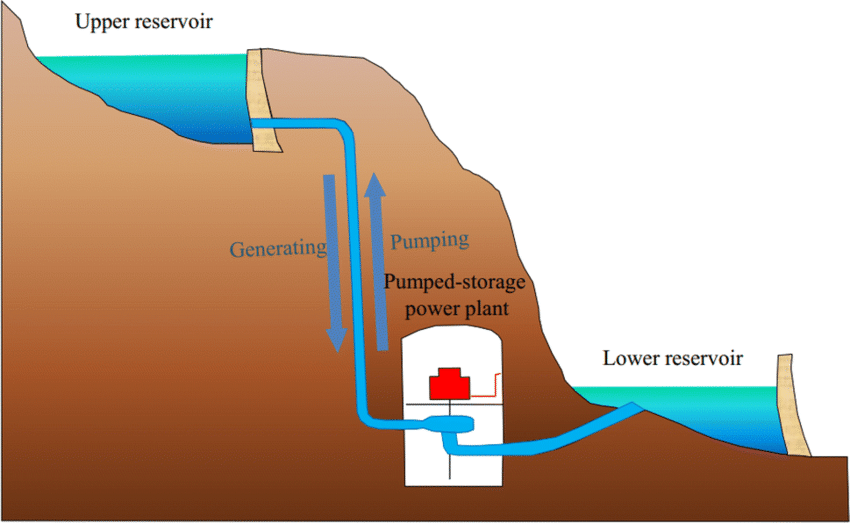
\includegraphics[width=\linewidth]{pumped_storage}
\end{center}
}

\headerbox{4. Computations}{name=screen,span=2,column=1,below=introduction}{ % To reduce this block to 1 column width, remove 'span=2'

We will simplify matters and consider a pyramid shaped reservoir. This is not an absolutely correct way of representing a reservoir, but it is easy and a good approximation of the order of magnitude. We will consider that the wall is 500 meters high (that's really, really high, more than twice as high as the great Game Of Thrones Wall), the sides (valley width) are approximately 2 kilometers apart, and the length (valley length used) around 5 kilometers. This gives us an upper reservoir that clocks in at 2 cubic kilometers volume of water. We will ignore the lower reservoir wall in our calculations (maybe it's a large natural lake, or even the ocean).

For a 500 meters high wall, and the 2 cubic kilometer reservoir discussed in our hypothetical facility, we have a potential energy of:

\begin{equation}\label{potential_energy}
E(V,h) = mgh = V \text{ ($m^3$)} * 1000 \text{ (kg/$m^3$)} * 10 \text{ (m.$s^{-2}$)} * h \text{ (m)}
\end{equation}

Note that $V$ varies with $h$.

\begin{equation}\label{potential_energy_2}
E(V(500),500) = 1 \times 10^{16} \text{ J} \approx 3 \text{ TWh}
\end{equation}

}

\headerbox{5. Results and Limitations}{name=sea,span=2,column=1,below=screen}{ % To reduce this block to 1 column width, remove 'span=2'

Recall that we need to have a energy storage capacity of around 40 TWh to meet France needs. We consequently need to build around 13 of those facilities.

Even the idea of the construction of \textit{just one} facility of this magnitude has never been entertained before. I personally cannot grasp the engineering effort needed to build a dozen, without international contributions (as every country would have to develop their program), on top of the grid transition itself.

We could drop the wall height requirements. Say you drop the 500 meters to 200 meters, giving you access to more sites and having an easier time building them. This means that the energy for each station would be around $E=0.4 \text{ TWh}$. You would need almost 100 of those, and 200 meters is not that small either (that's around the size of the Hoover dam).

Another thing to consider is the amount of land that would need to be flooded to create the upper reservoirs. The scenario with the 200 meter wall we considered represents a lake of around 5 square kilometers each on the surface, so a total area of 500 square kilometers. So, to cover the needs of France, that's around the size of Lake Geneva, that you have to create, foregoing the lower reservoir requirements.


\begin{kaobox}[frametitle=Common Questions]
\begin{itemize}
\item \textit{What about a larger number of smaller pumped hydroelectric storage stations?}

As we have seen going from 500 meters to 200 meters, it doesn't scale down linearly. We could drop the wall height requirements. Say you drop the 500 meters wall even further to 50 meters, giving you access to more sites. Now, the energy storage capacity for each station would be around $E=0.03 \text{ TWh}$. You would need almost 1500 of those. Good luck.

\item \textit{What about using the existing hydroelectricity power plants?}

France has 7.5 billion cubic meters of water available in its reservoirs.
%https://www.edf.fr/en/the-edf-group/producing-a-climate-friendly-energy/doubling-the-share-of-renewable-energies-by-2030/hydroelectric-energy/our-vision/environmental-issues/water-management-4
We assume that all reservoirs have a depth of 100 meters, which is a pretty generous assumption. The total capacity is thus around 2 TWh. Quite a way to go to 40 TWh.


\item \textit{It's not all about the height of the wall, is it?}

No, the height is used as a proxy to illustrate. You can see in the figure on the left panel that the feed pipes drops much more than the wall height. This can make dams more efficient. Don't hold your breath though, this take a very specific geology and geography to implement, and while it would help, it's not a game changer.

\end{itemize}
\end{kaobox}

}


\headerbox{6. Conclusions}{name=conclusion,column=1,below=sea,span=2,above=bottom}{
% DeCAF is a chemoinformatical tool that can be helpful in ligand-based drug design.
% It provides a comprehensive molecule description and a fast algorithms for comparing and aligning multiple ligands.
\begin{boenumerate}\compresslist
    \item Hydroelectric power has existed for a long time and represents today the main source of clean (along with nuclear) and renewable (alone) energy. 
    \item Creating projects required to power France need in storage would represent a gargantuan effort of epic proportions.
    \item The infrastructure already exists in prime locations, as long as we can create a lower reservoir to pump from, but the potential is not sufficient by an order of magnitude.
\end{boenumerate}
}


\headerbox{7. Go further}{name=references,column=0,span=1,below=mcs,above=bottom}{
Link to the Pumped Storage Case Study

Link to the Materials limitation Case Study

}

\end{poster}

\end{document}
